\lhead{Background}
\chapter{Background}
\label{Background}
	
	This chapter provides an overview of background knowledge which are necessary for understanding the content presented in this thesis. The outset of this chapter, \cref{Background:OceanEnvironmentModeling}, contains a brief discussion of the author's modeling choices for the ocean environment. These choices would lead to extensive use of Gaussian process models, whose mathematical background is detailed in \cref{Background:GaussianProcesses}. Path planning formulations, especially partially observable Markov decision processes, are motivated and discussed in \cref{Background:PathPlanning}.
	
	\section{Ocean Environment Modeling}
	\label{Background:OceanEnvironmentModeling}
	
		This thesis project can be broken down into two main parts - ocean environment modeling and path planning. Ocean environment modeling itself includes bathymetric feature extraction and modeling, and environment label modeling. This section will focus on the environment modeling aspect.
			
		In order for autonomous underwater vehicles to plan a path that can maximise the amount of information gained regarding a particular ocean region, it would need a method to predict the types of environments it may encounter, with a measure of its prediction uncertainty.
		
		While the path planner is to plan in the spatial space, in general the prediction model operates upon some feature space with more direct and explicit relationships with the output we would like to predict.
		
		It is thus important to make a distinction between the feature space $F$ for which label modeling is to occur and the spatial space $S$ for which bathymetric modeling and planning is to occur. The spatial space usually consists of Cartesian coordinates $(x, y)$ in the eastings-northings frame or the longitude-latitude frame. The path is to be planned in this spatial space. The frame is usually converted into a local body frame during the execution of control signals for path tracking. However, this does not affect the formulation presented here. The feature space includes bathymetric features for which the labels will be modeled upon. Depending on the features employed for the modeling process, there are usually approximate analytical forms for extracting such features from raw depth observations.

		The following features in \cref{Background:OceanEnvironmentModeling:Table:Features} were chosen by the author for bathymetric modeling. 

		\begin{table}[h]
			\begin{center}
				\begin{tabular}{ |c|c|c| }
					\hline
					Feature Name & Feature Symbol & Feature Units \\
					\hline
					Depth & $h$ & m \\
					Slope (Small Scale) & $m_{s}$ & m/m \\
					Slope (Large Scale) & $m_{l}$& m/m \\
					Rugosity (Small Scale) & $r_{s}$ & $\mathrm{m^{2}/m^{2}}$ \\
					Rugosity (Large Scale) & $r_{l}$ & $\mathrm{m^{2}/m^{2}}$  \\
					\hline
				\end{tabular}
			\end{center}
	  	\caption{Bathymetric Features}
	  	\label{Background:OceanEnvironmentModeling:Table:Features}			
	  	\end{table}	
		
		The raw bathymetric data contains depth information at various spatial locations. Such data are often collected rather uniformly in approximate grid formations such that it is possible to calculate the ocean floor slope through finite differencing. The slope is divided into small scale and large scale variations, as marine environments - especially underwater habitats - often depend not only on the immediate slope but also slope variations on the larger scale. The same idea applies to rugosity, the measure of local height variations. The feature extraction process is detailed in \cref{Background:OceanEnvironmentModeling:FeatureExtraction}. 
		  
		Spatial coordinates are chosen to be excluded from the bathymetric feature set. For environment prediction purposes, it is expected that ecological habitats and geological sites exhibit no explicit relationship with the location of the site, and that its properties arise solely due to the local environment characteristics (features) of that site.
		
		\FloatBarrier			
		
		Figure \ref{Background:OceanEnvironmentModeling:Figure:modelingprocess} show a high level overview of the ocean environment modeling process. As bathymetric data is available in more quantities and distributed more uniformly, it is often sufficient to employ the feature extraction process outlined in \cref{Background:OceanEnvironmentModeling:FeatureExtraction} to obtain the bathymetric features for modeling. However, if the bathymetric data is sufficiently sparse or is not distributed uniformly for grid based methods, then the feature extraction process itself becomes a prediction problem.

		\begin{figure}[!htbp]
			\centering
				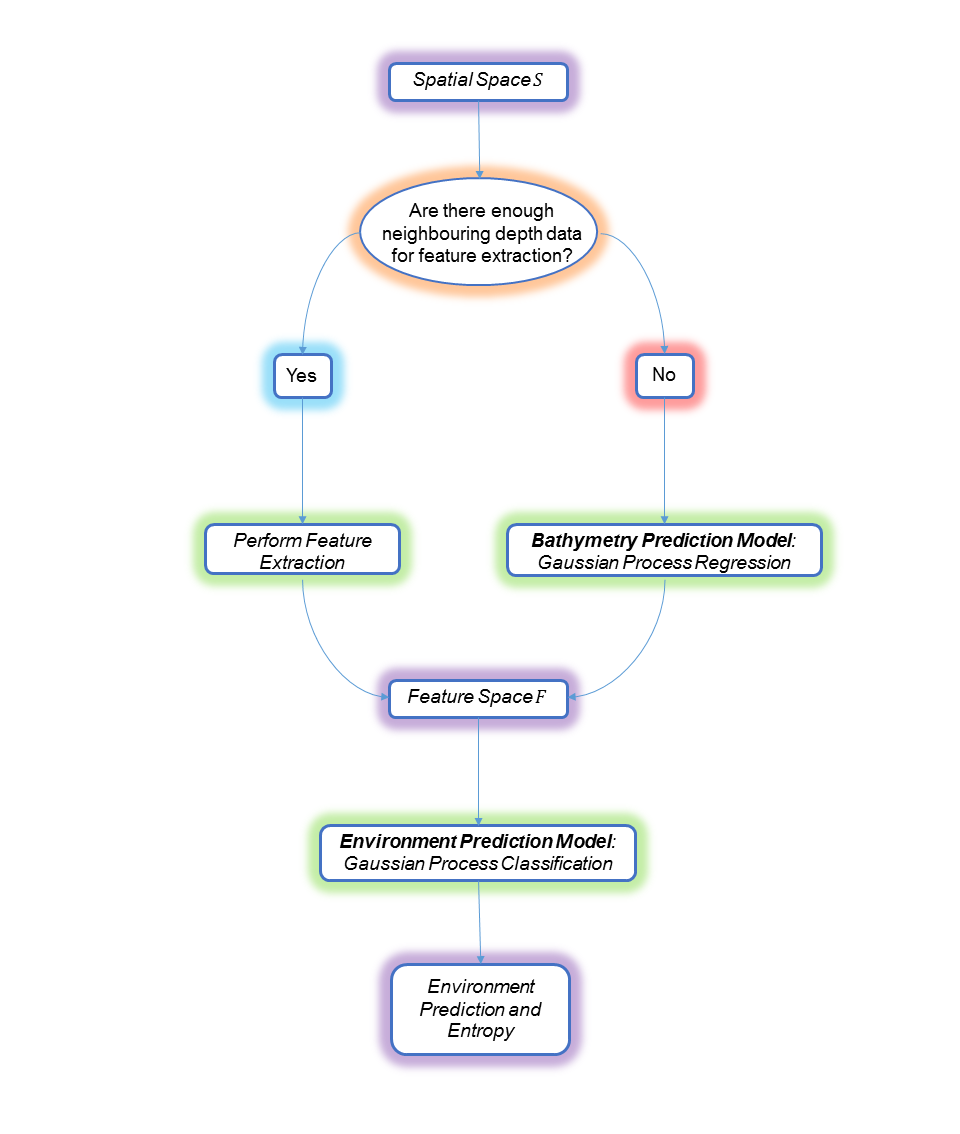
\includegraphics[width=\textwidth]{Figures/modelingprocess.png}
			\caption{Environment Modeling}
			\label{Background:OceanEnvironmentModeling:Figure:modelingprocess}
		\end{figure}
				
		In that case, a Gaussian process regression model is proposed for predicting the features at a given spatial location. While this is much more computationally expensive than performing feature extraction, it is also quite rare that this is necessary under abundant bathymetric data.
		
		Finally, once the feature vectors are obtained at training locations, the environment type is to be predicted. The environment type is summarised through labels that indicate the type of marine environment that was observed or predicted. Common AUV mission examples include "reef", "sand", and "rocks". These labels are often summarised through processing visual and stereo imagery obtained through past AUV missions. With a discrete set of possible labels, the environment prediction problem is to be modeled as a Gaussian process classification problem. From here on, the environment prediction problem is understood to refer to the two stage process of feature extraction or modeling and environment label prediction, with the latter being the main bottleneck for this process.
		
		\FloatBarrier
		
		\subsection{Environment Modeling - Data Matching}
		\label{Background:OceanEnvironmentModeling:DataMatching}
		
			A subtlety that arises from the above formulation is that during the training stage, the bathymetric data and the label data are not necessarily observed at the same places. Figure \ref{Background:OceanEnvironmentModeling:Figure:illustrationBathymetricAgainstLabels} illustrates the spatial distribution of the two datasets in a typical setting.
		
			\begin{figure}[!htbp]
				\centering
					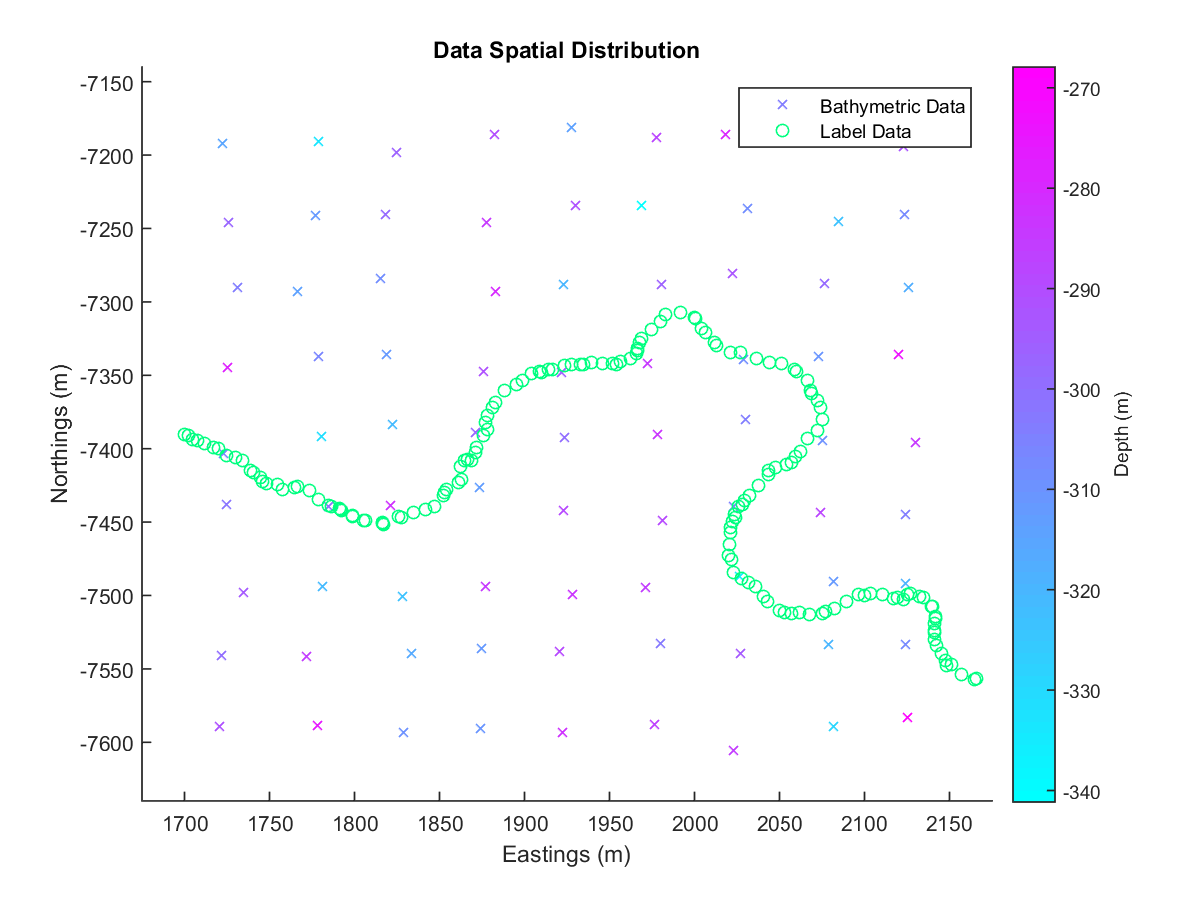
\includegraphics[width=0.9\textwidth]{Figures/illustrationBathymetricAgainstLabels.png}
				\caption{Illustration of Bathymetric and Label Data Density}
				\label{Background:OceanEnvironmentModeling:Figure:illustrationBathymetricAgainstLabels}
			\end{figure}
			
			While bathymetric data are usually collected rather uniformly, the label data are collected from past AUV missions whose trajectory are continuous curves across the ocean floor \cite{Squidle}. Due to slower AUV velocity as compared to surface ships which often employ SONAR or LIDAR techniques for bathymetry mapping, the label data are also spatially denser and concentrated on the mission trajectory, while being almost non-existent elsewhere.
			
			Therefore, in order to predict label data, the training data would need to be matched accurately. There are two straight forward choices at hand. The first is to estimate the bathymetric features at places where label data exists. However, at places near past mission paths, bathymetric data appears much more sparsely than label data, so that the feature extraction or regression prediction will yield very similar features across manly label data points. This reduces prediction power through a slow varying and limited feature group.
			
			Instead, the second choice is to estimate the label data at places where bathymetric data exists. In this setting, regions closer to past mission paths have higher volumes of label data, increasing the amount of training points. Regions further away would naturally generate more prediction uncertainty in the prediction stage.
			
			Hence, second method is chosen to be employed for data matching, in order to form our training set. Naturally, to predict environment labels from bathymetric features, we again need the Gaussian process classification model.
			
			\FloatBarrier
	
		\subsection{Feature Extraction}
		\label{Background:OceanEnvironmentModeling:FeatureExtraction}
		
			The feature extraction process assumes that the bathymetric depth data is available in grid form. That is, one can represent the available depth data $H = \{h_{k}\}_{k \in {1, 2, ..., N}}$ as $H = \{h_{ij}\}_{i \in {1, 2, ..., n_{i}}, \;\; j \in {1, 2, ..., n_{j}}}$ where varying $i$ and $j$ corresponds to varying data points in axis 1 and 2 respectively. Axis 1 and 2 is required to form an orthonormal frame. While axis 1 and 2 is usually aligned with the eastings-northings frame, it is generally not required for the feature extraction process.
			
			Without loss of generality, let $x$ and $y$ denote quantities corresponding to the orthogonal axes. We have that at $(x_{i}, y_{j})$ $(i \in {1, 2, ..., n_{i}}, \;\; j \in {1, 2, ..., n_{j}})$ the depth is measured as $h_{ij}$. The partial derivatives of various degrees of accuracy and scale can then be estimated through central differencing, as shown in \cref{Background:OceanEnvironmentModeling:Figure:centraldifferencecofficients} \cite{CentralDifferenceTable}. The author has chosen $N = 3$ neighbors for short scale slope and $N = 9$ neighbors for large scale slope.
			
			\begin{figure}[!htbp]
				\centering
					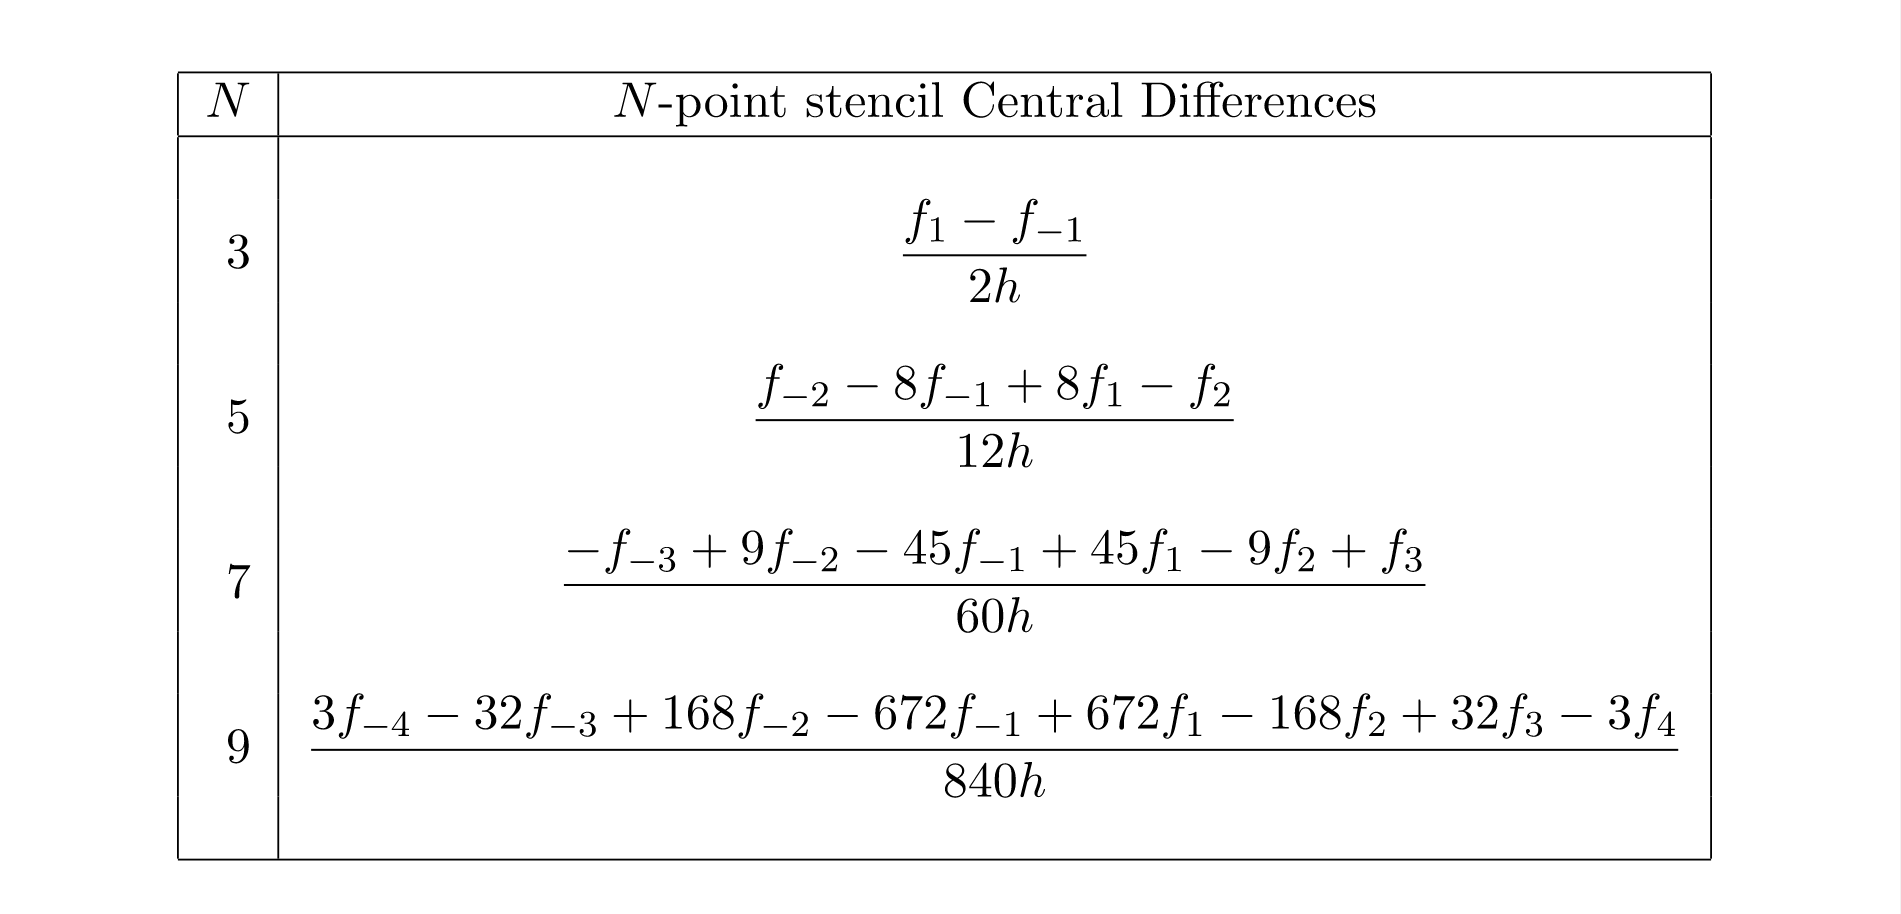
\includegraphics[width=0.9\textwidth]{Figures/centraldifferencecofficients.png}
				\caption{Finite Difference Methods: Central Difference Coefficients \\
				The subscripts $i$ represents  }
				\label{Background:OceanEnvironmentModeling:Figure:centraldifferencecofficients}
			\end{figure}			

			Central differencing is chosen as it is more numerically accurate. The disadvantages of instability and slightly higher time complexity from dynamic cases are not present in the static feature extraction process. Nevertheless, forward differencing is to be used at the boundaries of the dataset where neighboring data is missing on one side.
						
			With two axis, the result is a 2 element gradient vector. It is possible to treat the 2 elements as separate features. However, this would make the modeling problem frame dependent unnecessarily. Therefore, the magnitude of this gradient vector is taken as the slope feature. 
			
			Rugosity is a measure of local height variations in the terrain. By definition, its form is computed as $r = A_{r}/A_{g}$, the real surface area divided by the geometric surface area.
			
			Under cases without perfect grid formation, such as that shown in \cref{Background:OceanEnvironmentModeling:Figure:illustrationBathymetricAgainstLabels}, this feature extraction process becomes only an approximation. As the data set deviates from the form assumed above, it can then become necessary to estimate the features using Gaussian process regression - specifically, the multi-task Gaussian process regression. 
			
		 	On the other hand, under fine-scale bathymetric reconstructions, more sophisticated methods for deriving multi-scale measures of rugosity and slope exist. For example, under bathymetry measurements that are geo-referenced through stereo imagery, rugosity can be calculated through a Delaunay triangulated surface mesh and projecting areas onto the plane of best fit using Principal Component Analysis (PCA) \cite{StefanWilliams:Rugosity}.
							
			\FloatBarrier
			
	\section{Gaussian Processes}
	\label{Background:GaussianProcesses}
	
		Gaussian processes ($\mathcal{GP}$) are stochastic processes which generalises the multi-variate Gaussian distribution. In a statistical learning and machine learning context, they are categorised as a type of \textit{supervised learning} method, which describes the problem of learning relationships between input and output variables from empirical data. The empirical data is also often referred to as the training set.
		
		Supervised learning methods are often further categorised into regression and classification problems, depending on the nature of the output variable. The problem is a regression problem if the output is continuous, and a classification problem if the output is discrete. In the ocean environment modeling setting, bathymetric modeling is a regression problem (when feature extraction is infeasible), and environment type prediction is a classification problem.
		
		In both regression and classification settings, the input variables are often also referred to as \textit{features}, which motivated the term "bathymetric features" in the previous sections - especially to distinguish it from the spatial inputs. In statistical literature, continuous regression outputs are sometimes called \textit{response} variables, although it is more often simply referred as the \textit{output} or \textit{target} in the machine learning community. Discrete classification outputs are referred to as \textit{labels}. In this context, \textit{environment type} and \textit{environment labels} are synonymous. 
		
		In the sections which references the use of Gaussian process models, $\bvec{x}$ will denote the input variable or features of the problem while $y$ will denote the output or target variable. Note that in general there are multiple features such that the input is a feature vector $\bvec{x}$. Without loss of generality, however, the output variable can always be treated as a scalar quantity $y$. Under cases of multiple output variables, the problem can be split into multiple single output variable problems. It is true that prediction performance can actually be improved by considering the output vector together, which leads to multi-task regression, as will be briefly discussed. Nevertheless, the main bulk of the content revolve around single output Gaussian processes.
		
		The work presented here will be primarily based on Rasmussen and William's work in \textit{Gaussian Process for Machine Learning} from 2006 \cite{GaussianProcessForMachineLearning}. 
	
		\subsection{Bayesian Modeling and Gaussian Process}
		\label{Background:GaussianProcesses:BayesianModeling}
		
			The Gaussian process formulation follows the Bayesian modeling philosophy. An important distinction Bayesian modeling makes from the classical approach is the idea of estimating a distribution instead of a point value. While this is often more computationally expensive, it provides a very robust and accurate framework for prediction and analysis. More importantly, it provides capabilities that classical approaches do not possess - the ability to quantify prediction uncertainties. 
			
			The basic Bayesian modeling process begins with a prior distribution $p(H)$, the probability distribution of prediction model $H$ being representative, and updates this to a posterior distribution $p(H | D)$, the updated probability distribution of prediction model $H$ being representative after observing a particular data set $D$ \footnote{This discussion employs the common notational convention that the event of observing $D$ is also named $D$, and the event of model $H$ being the most representative is also named $H$.}. 
			
			This procedure is illustrated in \cref{Background:OceanEnvironmentModeling:Figure:bayesianmodeling}, where the posterior is updated by two observations. This example further serves to illustrate the concept of distributions over functions, which behaves as an infinite-dimensional generalisation of a multi-variate probability distribution. Instead of drawing random finite vectors from distributions, a random function is drawn from a \textit{process}, a term used to refer to infinite \footnote{When the input variable is temporal, a process can be more realistically interpreted as having indefinite dimensional distributions.} dimensional multi-variate distributions. It is helpful to conceptualise functions as an infinite string of points, such that drawing from an infinite dimensional distribution is equivalent to drawing from processes that operate on function space.
			
			\begin{figure}[!htbp]
				\centering
					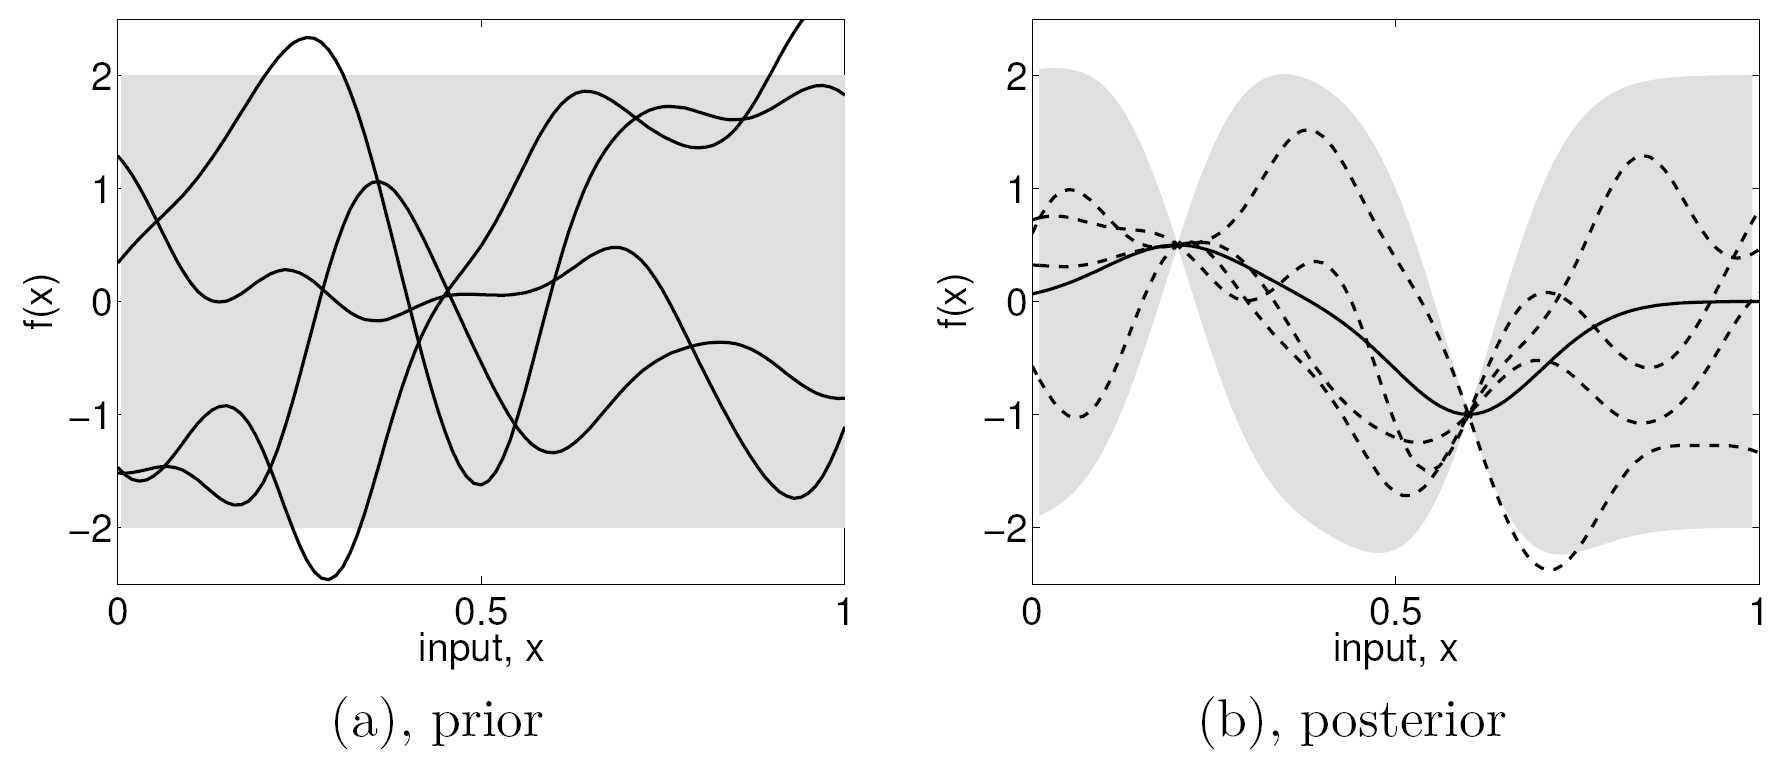
\includegraphics[width=0.9\textwidth]{Figures/bayesianmodeling.png}
				\caption{Illustration of Gaussian Process Bayesian Modeling: The mean prediction is shown as the solid line. Four samples are drawn in each case, represented by the dashed line. The shared region represents the 2-$\sigma$ bounds of the prediction at each input feature value $x$. Two points are observed which updated the distribution from the prior to the posterior.\\
				Figure (a) shows the situation for the prior distribution.\\
				Figure (b) shows the situation for the posterior distribution. \\
				Source: Rasmussen and Williams (2006) \cite{GaussianProcessForMachineLearning}}
				\label{Background:OceanEnvironmentModeling:Figure:bayesianmodeling}
			\end{figure}
			
			From this illustration, there are a few qualities one can notice. Firstly, the prior distribution is simply the zero function. The prior is meant to represent the system's current belief before the next observations are to be made. In this case, the prior situation involves no observations at all. Ideally, this means that the prior distribution should contain no predictive information. However, it is of philosophical note that all informative \footnote{It is certainly possible to perform inference without any assumptions. It will simply be uninformative in prediction or result.} inferences must start off with some assumptions regarding the structure of this problem. In the illustration above, the function is assumed to be distributed as a process with zero mean. This assumption has excluded processes without means, such as the Cauchy process, as well as assumed a rather arbitrary mean function. However, this assumption is often valid as one can always pre-process the output data set through subtracting off their empirical mean so that the output is distributed about zero. The representation of the variance functions as confidence bounds centered at the mean function also hints that multi-model processes are excluded. In fact, the illustration shows a Gaussian process, which is indeed uni-modal - just as its finite dimensional form.
			
			Speaking of the variance, a second observation is that the standard deviation and hence variance of the output function decreases at the observations, and gradually increases away from the observations. This leads to two remarks. Firstly, the variance or uncertainty of the output function at a location reduces when observations are made at that location. Secondly, neighboring points are related - the closer they are, the more related they are. This is seen through the observed points dragging nearby points towards it while reducing the uncertainty of nearby points. This resembles the concept of covariance. Evidently, points closer to each other have higher covariance then those further away, and the covariance beween the same points simply become its variance.
			
			The two observations above demonstrate that, just as a Gaussian distribution is defined through a mean vector and a covariance matrix, a Gaussian process is defined through a mean function $m(x)$ and a covariance function $k(x, x')$. In Gaussian process literature, the covariance function is also called a \textit{kernel} function.
			
			Formally, a function $f(x)$ is distributed as a Gaussian process $f(x) \sim \mathcal{GP}(m(x), k(x, x'))$ if for any finite collection of points $\bvec{x} := [x_{1}, x_{2}, \dots, x_{n}]^{T}$, the corresponding output vector $f(\bvec{x}) := [f(x_{1}), f(x_{2}), \dots, f(x_{n})]^{T}$ is jointly distributed as a multi-variate Gaussian such that $f(\bvec{x}) \sim \mathcal{N}(\bvec{m}(\bvec{x}), K(\bvec{x}, \bvec{x}'))$. Certainly, this is true for finite dimensional multi-variate Gaussian distributions, in that any subset of a said distributed random vector will also be multi-variate Gaussian distributed of lower dimensionality. The next few sections will discuss the kernel matrix $K$ more rigorously.
			
			Finally, as mentioned before, the mean function can be generally assumed to be the zero function, as at each stage of inference both the model and data can be subtracted by their theoretical or empirical means. This elucidates that Gaussian processes are completely defined by their kernel function $k$. 
			
			\FloatBarrier
			
		\subsection{Kernel Functions}
		\label{Background:GaussianProcesses:KernelFunctions}
		
			As kernel functions completely define the prediction characteristics of a Gaussian process, this section aims to provide the mathematical background regarding kernels that are necessary for understanding Gaussian processes. The following discussion will only cover the minimal background necessary for further sections, as treatments of kernel functions can easily become very detailed and rigorous once analysis begins in topics such as differentiability effects or eigenfunction decomposition. Further treatment of this material is available through Rasmussen and Williams (2006) \cite{GaussianProcessForMachineLearning}. 
			
			Intuitively, the kernel function determines the \textit{similarity} between data points. This is a notion that all supervised learning algorithms intend to do, although rather implicitly in most cases. The $\mathcal{GP}$ formulation makes this explicit through the covariance between any two points in the feature space.
			
			Kernel functions can be categorised into stationary kernels and non-stationary kernels. In this thesis, non-stationary kernels will become of vital importance in bathymetric and environment modeling. 
			
			Stationary kernels are ones whose covariance properties do not depend explicitly on the locations $\bvec{x}$ and $\bvec{x}'$ of consideration, but only on the difference $\bvec{x} - \bvec{x}'$ between them. Thus, the covariance properties are \textit{stationary}, or invariant, under translations in the feature space.
			
			Common stationary kernels are the squared exponential kernel \footnote{Squared exponential kernels are also sometimes called Gaussian kernels. However, in conversations it tends to create confusion between the probability density function $\phi(x)$ for Gaussian distributions and the covariance function $k(x, x')$ itself, so this term is avoided in this thesis.} and the \matern kernels. The squared exponential (SE) kernel between any two points $\bvec{x}, \bvec{x}' \in \mathbb{R}^{m}$ in the feature space with $m$ features has the following form \eqref{Background:GaussianProcess:Equation:SquaredExponentialKernel}.
			
			\begin{equation}
				\left.
					\begin{aligned}
						k_{\mathrm{SE}}(\bvec{x}, \bvec{x}') &= \sigma_{f}^{2} \exp\Big(-\frac{1}{2}(\bvec{x} - \bvec{x}')^{T} \Sigma^{-1} (\bvec{x} - \bvec{x}')\Big) = \sigma_{f} \exp\Big(-\frac{1}{2} a^{2} \Big) \\
						\Sigma &= 	\begin{bmatrix}
										l_{1}^{2} & l_{12} & \dots & l_{1m} \\
										l_{21}^{2} & l_{2}^{2} & \dots & l_{2m} \\
										\vdots & \vdots  & \ddots & \vdots \\
										l_{m1}^{2} & l_{m2} & \dots & l_{m}^{2} \\
								  	\end{bmatrix}
					\end{aligned}
				\qquad \right.
			\label{Background:GaussianProcess:Equation:SquaredExponentialKernel}
			\end{equation}
			
			Here, $\sigma_{f}$ is called the sensitivity, and determines the overall reference strength scale of the covariance function. The matrix $\Sigma$ is the length scale matrix, and determines the reference length scale and principle axis directions within the feature space. Like most quadratic forms, $\Sigma$ is required to be symmetric and positive semi-definite. In particular, when $\Sigma$ is diagonal, the kernel is termed \textit{axis aligned}. When $\Sigma$ is proportional to an identity such that $\Sigma = l^{2} I_{m \times m}$, the kernel is termed \textit{isotropic}.
			
			The sensitivity parameter $\sigma_{f}$ and length scale parameters $l_{ij}$, $i, j \in {1, 2, \dots, m}$ with $l_{i} := l_{ii}$ completely withhold the information of a squared exponential kernel. Unlike parametric models, however, while these parameters define the kernel directly, they define the $\mathcal{GP}$ model indirectly. Because of the multiple levels of relation from these parameters to the model, these parameters are termed \textit{hyperparameters} of the $\mathcal{GP}$.
			
			In practice, it is often possible to pre-process the data or transform the feature space so that an axis aligned kernel can be applied. The assumption imposed is that the principle axis directions are aligned with the feature space axis. In this case, the $\mathcal{GP}$ model is defined by $m + 1$ hyperparameters, where $m$ is the number of features. Even without the axis-aligned assumption, the number of hyperparameters is $\frac{m(m + 1)}{2} + 1$.
			
			The above formulation suggests to define $a^{2} := (\bvec{x} - \bvec{x}')^{T} \Sigma^{-1} (\bvec{x} - \bvec{x}')$. This can be interpreted as the squared distance between $\bvec{x}$ and $\bvec{x}'$ under the warp defined by $\Sigma$. In particular, when the feature space is isotropic such that $\Sigma = l^{2} I_{m \times m}$, then $a = \frac{r}{l}$ where $r := +\sqrt{r^{2}}$, $l := +\sqrt{l^{2}}$, and $r^{2} = (\bvec{x} - \bvec{x}')^{T} (\bvec{x} - \bvec{x}')$. In fact, most stationary kernels are functions solely of $a^{2}$, or with the definition $a := +\sqrt{a^{2}}$, they are simply scalar functions with scalar inputs $a = a (\bvec{x}, \bvec{x'})$. This form also makes evident that the covariances between two points decreases monotonically as the distance between them increases - a property most kernel functions exhibit.
			
			Continuing with this formulation, the \matern class of kernel functions are given by \eqref{Background:GaussianProcess:Equation:MaternKernel}.
			
			\begin{equation}
				\left.
					\begin{aligned}
						k_{\mathrm{\maternmath}}(\bvec{x}, \bvec{x}') =& \; \sigma_{f}^{2} \frac{2^{1 - \nu}}{\Gamma(\nu)} \Big( \sqrt{2 \nu} a \Big)^{\nu} K_{\nu}\Big( \sqrt{2 \nu} a \Big) \\
						a^{2} :=& \; (\bvec{x} - \bvec{x}')^{T} \Sigma^{-1} (\bvec{x} - \bvec{x}')
					\end{aligned}
				\qquad \right.
			\label{Background:GaussianProcess:Equation:MaternKernel}
			\end{equation}
						
			$\Gamma$ and $K_{\nu}$ are the Gamma function and modified Bessel function respectively \cite{GaussianProcessForMachineLearning}. $\nu$ is a positive hyperparameter that determines the differentiability property of the \matern class kernel. The $\mathcal{GP}$ model with \matern class kernel is $d$-times mean square differentiable if and only if $\nu > k$. In the limit of $\nu \rightarrow \infty$ for infinite differentiability, the \matern kernel becomes the squared exponential kernel \eqref{Background:GaussianProcess:Equation:SquaredExponentialKernel}. While the general \matern class kernel seem complicated due to the Gamma function and modified Bessel function, its form become simple for $\nu = p + \frac{1}{2}$ where $p$ is a non-negative integer. That is, \matern kernels with $\nu = \frac{1}{2}, \frac{3}{2}, \frac{5}{2}, \frac{7}{2}, \dots$ have simple analytic forms without reference to the modified Bessel function. In fact, for $\nu > \frac{5}{2}$, the degree for which the \matern kernel changes becomes quite unnoticeable for most practical purposes such that it may as well be replaced by the squared exponential kernel with $\nu \rightarrow \infty$. Similarly, while there is a more noticeable effect of changing $\nu$ within the range $\nu \in (0, \frac{5}{2})$, in practice is it is often not worth the expense of implementing the complicated form for a almost unnoticeable improvement in modeling accuracy. Hence, it is replaced with the \matern kernel $\nu = \frac{1}{2}, \frac{3}{2}, \frac{5}{2}$, whichever is the closest. In this way, in practice only the \matern kernels with $\nu = \frac{1}{2}, \frac{3}{2}, \frac{5}{2}$ are employed, and they are respectively termed the \matern 1/2 kernel, \matern 3/2 kernel, and \matern 5/2 kernel - in the order of increasing differentiability. These kernels have forms as listed below \eqref{Background:GaussianProcess:Equation:PracticalMaternKernels}.
			
			\begin{equation}
				\left.
					\begin{aligned}
						k_{\mathrm{\maternmath}, \; \nu = \frac{1}{2}}(\bvec{x}, \bvec{x}') =& \; \sigma_{f}^{2} \exp ( -a ) \\
						k_{\mathrm{\maternmath}, \; \nu = \frac{3}{2}}(\bvec{x}, \bvec{x}') =& \; \sigma_{f}^{2} (1 + \sqrt{3} a) \exp ( -\sqrt{3} a ) \\
						k_{\mathrm{\maternmath}, \; \nu = \frac{5}{2}}(\bvec{x}, \bvec{x}') =& \; \sigma_{f}^{2} \Big(1 + \sqrt{5} a + \frac{5}{3} a^{2}\Big) \exp ( -\sqrt{5} a )  \\
						a^{2} :=& \; (\bvec{x} - \bvec{x}')^{T} \Sigma^{-1} (\bvec{x} - \bvec{x}')
					\end{aligned}
				\qquad \right.
			\label{Background:GaussianProcess:Equation:PracticalMaternKernels}
			\end{equation}			
			
			Together, the squared exponential kernel and the \matern class kernels provide a flexible set of kernel functions that can model a multitude of phenomena from various fields such as geology, ecology, finance, logistics, control theory, and machine learning. Specifically, kernel functions make spatial relations explicit which assists in the interpretation in spatial modeling cases, including bathymetric modeling and ocean environment modeling.
			
		\subsection{Regression}
		\label{Background:GaussianProcesses:Regression}
		
			Gaussian process regression is a regression technique that employs Gaussian processes as its inference model. Because Gaussian processes already operate on function spaces with continuous inputs and outputs, no extra pre-processing or transformations are needed. The bulk of the technique thus lies in learning the kernel function of the Gaussian process. Gaussian process regression is also called \textit{kriging} or Kolmogorov Wiener prediction when used for interpolating geospatial data in a geostatistics setting. This section attempts to summarise the important concepts regarding $\mathcal{GP}$ regression and how they work. More rigorous discussions are available from Rasmussen and Williams (2006) \cite{GaussianProcessForMachineLearning}. 
			
			Once a kernel function is chosen, such as the squared exponential or \matern kernels, learning the kernel function becomes equivalent to learning the hyperparameters of the kernel. In this way, the Gaussian process model is actually defined completely by its hyperparameters, which are often only handful in quantity. This illustrates that while its temporal complexity $\mathcal{O}(n^{3})$ is quite high, its spatial complexity and memory requirements are quite moderate at $\frac{m(m + 1)}{2} + 1 + n(m  + 1)$ real numbers, where $n(m  + 1)$ real numbers comes from the training data itself. % Minimally, after assuming a particular kernel functional form, the bulk of the model information is held by the data set itself. Especially in big data applications, unlike generalised linear models and neural networks whose information vector \footnote{The information vector is the vector of all parameters that defines the model.} is proportional to the number of basis functions employed, a Gaussian process model can have its information stored by a few hyperparameters.
			
			With a given kernel function $k$ as the covariance function, by definition we have that the training observations $\bvec{f}$ and the query observations $\bvec{f^{\star}}$ is distributed as a multivariate Gaussian \eqref{Background:GaussianProcess:Equation:Distribution}.
			
			\begin{equation}
				\begin{bmatrix}
					\bvec{f^{ }} \\ \bvec{f^{\star}}
				\end{bmatrix}
				\sim \mathcal{N}\Bigg(\bvec{0}, \begin{bmatrix}
													K(X, X) & K(X, X^{\star}) \\
													K(X^{\star}, X) & K(X^{\star}, X^{\star}) \\
												\end{bmatrix}  \Bigg)
			\label{Background:GaussianProcess:Equation:Distribution}
			\end{equation}
			
			where the matrix $K(X, X')$ is defined to have elements $K_{ij} = k(\bvec{x}_{i}, \bvec{x}'_{j})$ with $X$ and $X'$ defined as the canonical data design matrix form \eqref{Background:GaussianProcess:Equation:DataMatrix}, both of each can take either the matrix of training points $X$ of size $n$ or query points $X^{\star}$ of size $n^{\star}$. To shorten notation, it is customary to define $K := K(X, X)$, $K^{\star} := K(X, X^{\star})$, $K^{\star \star} := K(X^{\star}, X^{\star})$, where the symmetry of the covariance matrix readily yields ${K^{\star}}^{T} := K(X^{\star}, X)$. Specifically, $K$ will be referred to as the data kernel.
			
			\begin{equation}
				X = \begin{bmatrix}
					\bvec{x}_{1}^{T} \\ \bvec{x}_{2}^{T} \\ \dots \\ \bvec{x}_{n}^{T}
				\end{bmatrix} \qquad X' = \begin{bmatrix}
									\bvec{x'}_{1}^{T} \\ \bvec{x'}_{2}^{T} \\ \dots \\ \bvec{x'}_{n}^{T}
								\end{bmatrix}
			\label{Background:GaussianProcess:Equation:DataMatrix}
			\end{equation}	
				
			The joint distribution readily contains information for the conditional distribution of the query points given the training points $p(\bvec{f^{\star}} | \bvec{f})$ knowing the training points and query locations \footnote{Throughout this thesis, since the feature locations $X$ and $X^{\star}$ are always known, they are inherently conditioned upon and will not be shown explicitly in notation.}. This leads to the posterior distribution \eqref{Background:GaussianProcess:Equation:ConditionalDistribution}.
			
			\begin{equation}
				\bvec{f^{\star}} | \bvec{f} \sim \mathcal{N}({K^{\star}}^{T} K^{-1} \bvec{f}, K^{\star \star} - {K^{\star}}^{T} K^{-1} K^{\star})
			\label{Background:GaussianProcess:Equation:ConditionalDistribution}
			\end{equation}						
			
			A comparison with the prior $\bvec{f^{\star}} \sim \mathcal{N}(\bvec{0}, K^{\star \star})$ shows the mean effect ${K^{\star}}^{T} K^{-1} \bvec{f}$ and covariance effect $- {K^{\star}}^{T} K^{-1} K^{\star}$ which introduces observed information into the model. Interestingly, as ${K^{\star}}^{T} K^{-1} K^{\star}$ is positive definite, this intuitively means that the observation has reduced uncertainty in the model.
			
			The above posterior formulation encompasses the heart of the GP regression model. The rest of the discussion will focus on detailed aspects of its implementation and variants.
			
			\subsubsection{Noisy Observations}
			
				Under noisy observations, a hyperparameter $\sigma$ is introduced for the standard deviation of the noise, which is also assumed to be \textit{iid} and Gaussian distributed with standard deviation $\sigma$ and zero mean. The only alteration is the observations are notated as $\bvec{y}$ instead of $\bvec{f}$, and most importantly the data kernel is to be replaced with $K \mapsto K + \sigma^{2} I$. Note that however the query points remain as the latent function $\bvec{f^{\star}}$. If one were to predict future observations $\bvec{y^{\star}}$, then it suffices to generate $\bvec{f^{\star}}$ from the posterior and add randomly generated noise with standard deviation $\sigma$.
				
			\subsubsection{Learning the Hyperparameters}
			
				One of the most important yet tricky aspects of GP modeling is the training stage. Since the model is determined entirely by the hyperparameters, the hyperparameters must be optimised in accordance to some fitness metric. The fitness metric employed to be maximised is the marginal likelihood, otherwise termed as evidence, of the observed data. This is usually non-trivial to calculate and, in most cases, analytical forms do not exist. Fortunately, due to the Gaussian assumption of he GP model, there exists an analytical form for the marginal likelihood. In practice, however, it is computationally faster to compute the log marginal likelihood \eqref{Background:GaussianProcess:Equation:LogMarginalLikelihood}.
				
				\begin{equation}
					\log(p(\bvec{f})) = - \frac{1}{2} \bvec{f}^{T} K^{-1} \bvec{f} - \frac{1}{2} \log|K| - \frac{n}{2} \log(2 \pi)
				\label{Background:GaussianProcess:Equation:LogMarginalLikelihood}
				\end{equation}
				
				Again, with noisy observations, corresponding substitutions with the data kernel matrix $K \mapsto K + \sigma^{2} I$ and observations $\bvec{f} \mapsto \bvec{y}$ is to be made.
				
				The last term is a constant, so it can be ignored during the optimisation stage and included back in once optimisation completes.
				
				In practice, hyperparameter learning can be sped up by employing the fact that $\frac{1}{2} \log|K| = \sum_{i} L_{ii} = \mathrm{trace}(L)$ where $L$ is the Cholesky decomposition of $K$ (or $K + \sigma^{2} I$ in the noisy case). In fact, the Cholesky decomposition $L$ leads to better numerical stability when inverting the matrix $K$ since $K = LL^{T}$ so that $K \backslash \bvec{y} = L^{T} \backslash (L \backslash \bvec{y})$.
				
			\subsubsection{Multi-task Regression}
			
				Multi-task regression operates on the same principles as the single-task regression. With multiple outputs, each output is assigned to a single-task regression problem as discussed above. However, a covariance matrix between each output is kept track of such that each output can perform inference on other outputs as well.
				
				The advantage of this approach is that different outputs recorded at different feature positions can assist each other to fill in each other's data gap. In this way, the over all entropy can be reduced.
				
				In an environment modeling setting, the main problem that occurs even after a good model has been learned is that entropy always increases at places where there is less data, as opposed to places that are inherently interesting and high in entropy even after observations. Multi-tasking improves the situation by lowering the entropy at those places with scarce data but inherently uninteresting.
				
		\subsection{Classification}
		\label{Background:GaussianProcesses:Classification}
		
			The GP classification method is of vital importance to the environment modeling process. It is used to distinguish and predict the environment type with a measure of entropy in order to quantify the information reward one can gain by exploring the area.
			
			Unlike the regression case, because the output labels are no longer continuous, it cannot be represented by a continuous probability density function such as a Gaussian. As such, a continuous latent function is introduced in the GP classification process. Intuitively, this latent function quantifies and measures the distinct qualities of the label. As a binary classification example, if the classifier is to distinguish between "Apples" and "Oranges", the latent function would then represent the "Appleness" of each observation, with high "Appleness" corresponding to observations likely to be "Apples" and low "Appleness" corresponding to observations likely to be "Oranges". Note that only one latent function is needed in the binary case. The latent function is then "squashed" into the unit range [0, 1] so that it can be interpreted as a probability.
			
			Although the latent function is now continuous such that it is possible to model it with a GP regression model, the posterior probability is in general non-Gaussian distributed. In this way, approximations are necessary.
			
			There exists four approximate methods for GP classification. In increasing orders of accuracy and decreasing order of implementation difficulty, they are Probabilistic One Nearest Neighbor (P1NN), Laplace Approximation (LP), Expectation Propagation (EP), and Gaussian Process Least Squares Classifier (GPLSC) \cite{GaussianProcessForMachineLearning}. In this section, Laplace approximation is chosen as a reasonable balance between accuracy and implementation difficulty.
			
			\subsubsection{Response Functions}
			
				Before discussions begin regarding the various types of GP classifiers, it is important to understand the role of \textit{response functions} in Bayesian classifiers.
				
				The response function is sometimes also called a sigmoid function. These functions must satisfy the requirement that is it monotonically non-decreasing with a domain of all real numbers $\mathbb{R}$ and a range of unit interval [0, 1]. That is, $\lambda(z): \mathbb{R} \mapsto [0, 1]$. As referenced above, these functions serve to "squeeze" the latent functions into a range where probabilistic interpretation is possible.
				
				The most widely used response function is with no doubt the logistic function \eqref{Background:GaussianProcess:Equation:Logistic}. Response functions that are also commonly used in a GP classifier setting include the normal cumulative distribution function \eqref{Background:GaussianProcess:Equation:normalcdf}.
				
				\begin{equation}
					\lambda(z) = \frac{1}{1 + \exp(-z)}
				\label{Background:GaussianProcess:Equation:Logistic}
				\end{equation}
				
				\begin{equation}
					\lambda(z) = \Phi(z) := \int\limits_{-\infty}^{z} \phi(x) dx =  \int\limits_{-\infty}^{z} \frac{1}{\sqrt{2 \pi}} \exp\Big(- \frac{1}{2} x^{2}\Big) dx
				\label{Background:GaussianProcess:Equation:normalcdf}
				\end{equation}
				
			\subsubsection{Binary Classification}
			
				The Laplace approximation for GP binary classification works by learning a latent function through an iterative scheme involving successive GP regressions, and "squeezing" that latent function into an appropriate probabilistic range for likelihood interpretation. The Laplace approximation approaches the approximation problem by determining the mean and variance of the true distribution and approximating the said distribution with a Gaussian distribution of the same mean and variance. Assuming Gaussian distributions, the prior and the evidence (marginal likelihood) have analytical forms. Under such assumptions it is therefore possible to marginalise out the likelihood predictions to obtain a posterior estimate. Finally, this learning stage can be trained by optimising the marginal likelihood \footnote{{\color{BurntOrange} At this stage of the thesis progress, it is uncertain whether or not a deeper and more rigorous theoretical grounding should be provided for GP classification. Perhaps it would benefit by only providing an intuitive outline of the procedure, rather than a rigorous derivation, so that the reader is not distracted from the main contributions of this thesis later on.}}.
				
			\subsubsection{Multi-class Classification: One v.s. All and All v.s. All}
			
				While a consistent framework for the GP Multi-class classification using Laplace approximation exist, a simpler and perhaps a more computationally efficient approach is to employ the One v.s. All (OVA) and All v.s. All (AVA) philosophy. The following discussion assumes that there are $c > 2$ classes of labels for which classification is to occur. 
				
				The OVA approach performs classification by introducing $c$ \textit{independent} classification problems, each trying to classify a label against all others. Each of these problems are thus a binary classification problem for which solution methods are known. Once the predictive probabilities from all learned GP classifiers are obtained, a consistent framework is used for fusing the separate prediction probabilities into a coherent prediction probability. This is necessary as the binary classifiers are independently learned and performs prediction independently, and may not necessarily provide coherent results. In fact, simply stacking the prediction probabilities together yields a "probability" distribution that does not sum up to 1.
				
				The AVA approach operates similarly. It insteads introduces $\frac{c (c - 1)}{2}$ \textit{independent} classification problems, each classifying between a pair of labels. The same exact philosophy follows in that a final consistent framework is needed for fusing the prediction probabilities into one coherent prediction probability. It is often more difficult for probability fusion in the AVA setting as compared to the OVA setting.
				
			\subsubsection{Fusion of Prediction Probability}

				{\color{BurntOrange} This section should be in the GP implementation chapter of this thesis (e.g. Chapter 3). It would further the discussion above regarding the probability fusion problem by introducing the exclusion method and mode keeping method that has been developed and tested. It is anticipated that other methods will be developed by then, so that this section would undergo significant editing.}
				
%				The main decision and analysis to be made in both the OVA and AVA setting is the framework for which the probabilities are to be fused. 
%							
%				The exclusion method centers around the idea that the probabilities are to be made consistent by eliminating, or excluding, the events that are impossible.
%				
%				Consider a single query point for which class prediction is to occur. Let $\pi_{i}$ be the prediction probability obtained through the binary classification of class $i$ against all other classes. Initially, the probability vector $\bvec{\pi} := [\pi_{1}, \pi_{2}, \dots, \pi_{c}]^{T}$ is not a unit vector, so that $\bvec{\pi}$ does not define a proper probability distribution \dots 
		
			\subsubsection{Entropy}
			
				After a predictive probability distribution is obtained for each query environment location, the uncertainty of such predictions can be quantified through the entropy of of that distribution.
				
				The output of a GP classifier is a discrete probability distribution with finite size - equal to the number of classes. For a general discrete probability distribution $p(x)$, the entropy is quantified as below \eqref{Background:GaussianProcess:Equation:DiscreteEntropy}.
				
				\begin{equation}
					H(p(x)) = - \sum_{i} p(x_{i}) \log(p(x_{i}))
				\label{Background:GaussianProcess:Equation:DiscreteEntropy}
				\end{equation}
				
				Although it is unlikely that the entropy of bathymetric feature modeling is required, the regression posterior is a continuous probability density $p(x)$ for which a similar form for distribution entropy exists \eqref{Background:GaussianProcess:Equation:ContinuousEntropy}.
				
				\begin{equation}
					H(p(x)) = - \int_{\Omega_{x}} p(x) \log(p(x)) dx
				\label{Background:GaussianProcess:Equation:ContinuousEntropy}
				\end{equation}
								
				With these entropy measures, predictive uncertainties can be quantified, which allows active information seeking plans to be possible.
				
		\subsection{Non-Stationary Kernels}
			
			Non-stationary kernels introduce flexibility for modeling phenomenons where the inherent length scales varies across feature locations. The problem with stationary kernels is that the GP will always learn length scales that are as small as it needs to for modeling the fastest varying phenomenon in the model. While the marginal likelihood inherently balances modeling accuracy and overfitting, when it comes to the choice between modeling a peak in data variation with a risk of overfitting the rest of the data or ignoring that peak, the optimiser will always prefer the former as marginal likelihood gain from successful modeling is higher than loss from overfitting. Because learning stage is done through optimising the marginal likelihood, this forces the length scale to be smaller than it needs at slower varying places.

			Figure \ref{Background:GaussianProcess:Figure:gaussianprocesslengthscale} illustrates the non-stationary Gaussian process for a terrain modeling application. Note that this does not imply that it is only relevant for GP regression problems - the latent functions used in GP classification is itself a GP regression problem for which length scale interpretation is almost identical to that shown in \cref{Background:GaussianProcess:Figure:gaussianprocesslengthscale}.
			
			\begin{figure}[!htbp]
				\centering
					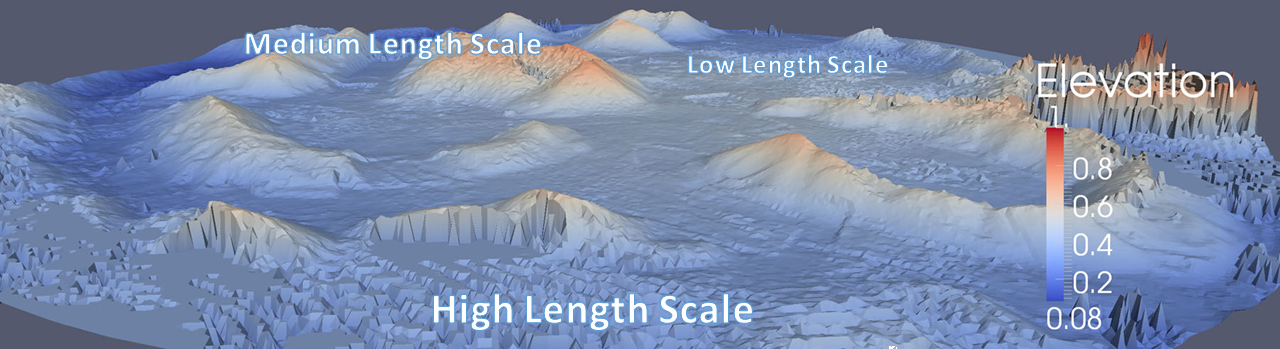
\includegraphics[width=\textwidth]{Figures/gaussianprocesslengthscale.png}
				\caption{Illustration of non-stationary Gaussian process for terrain modeling \cite{GaussianProcessTerrainFigure} \\
				Flat parts have high length scales (slow varying) while \\ rough parts have low length scales (fast varying)}
				\label{Background:GaussianProcess:Figure:gaussianprocesslengthscale}
			\end{figure}
			
			The non-stationary kernel function employed is the Paciorek Non-Stationary Covariance Function \eqref{Background:GaussianProcess:Equation:NonStationaryKernel} \cite{AdaptiveNonStationaryKernel}.
			
			\begin{equation}
				k(\bvec{x}_{i}, \bvec{x}_{j}) = \sigma_{f}^{2} |\Sigma_{i}|^{\frac{1}{4}} |\Sigma_{j}|^{\frac{1}{4}} \Bigg|\frac{\Sigma_{i} + \Sigma_{j}}{2}\Bigg|^{-\frac{1}{2}} \exp\Bigg[ -\frac{1}{2} (\bvec{x}_{i} - \bvec{x}_{j}) \Bigg(\frac{\Sigma_{i} + \Sigma_{j}}{2}\Bigg)^{-1} (\bvec{x}_{i} - \bvec{x}_{j}) \Bigg]
			\label{Background:GaussianProcess:Equation:NonStationaryKernel}
			\end{equation}			
			
			The matrices $\Sigma_{i}$ and $\Sigma_{j}$ are the local length scale matrices at $\bvec{x}_{i}$ and $\bvec{x}_{j}$ respectively, and are interpreted the same way as the stationary case. The only difference is that these length scale matrices only operate locally, and are functions of the input feature vector $\bvec{x}$. In each kernel location, two length scale matrices are queried. Hence, in a kernel matrix of size $n \times m$, around $n + m$ unique queries are made if no feature locations overlap.
			
			It is worthwhile to observe that the effective length scale matrix in the exponent is the average of the two length scale matrices, with its effect reduced with increasing distance between the two points of consideration as with all kernels.
			
			Note that the normalisation matrix determinants are chosen such that the kernel function is reduced into a stationary one when $\Sigma_{i} = \Sigma_{j} = \Sigma$ \eqref{Background:GaussianProcess:Equation:NonStationaryKernelToStationary}. 
			
			\begin{equation}
				\left.
					\begin{aligned}
						k(\bvec{x}_{i}, \bvec{x}_{j}) &= \sigma_{f}^{2} |\Sigma|^{\frac{1}{4}} |\Sigma|^{\frac{1}{4}} \Bigg|\frac{\Sigma + \Sigma}{2}\Bigg|^{-\frac{1}{2}} \exp\Bigg[ -\frac{1}{2} (\bvec{x}_{i} - \bvec{x}_{j}) \Bigg(\frac{\Sigma + \Sigma}{2}\Bigg)^{-1} (\bvec{x}_{i} - \bvec{x}_{j}) \Bigg] \\
						k(\bvec{x}_{i}, \bvec{x}_{j}) &= \sigma_{f}^{2} |\Sigma|^{\frac{1}{2}} |\Sigma|^{-\frac{1}{2}} \exp\Bigg[ -\frac{1}{2} (\bvec{x}_{i} - \bvec{x}_{j}) (\Sigma)^{-1} (\bvec{x}_{i} - \bvec{x}_{j}) \Bigg] \\
						k(\bvec{x}_{i}, \bvec{x}_{j}) &= \sigma_{f}^{2} \exp\Bigg[ -\frac{1}{2} (\bvec{x}_{i} - \bvec{x}_{j}) \Sigma^{-1} (\bvec{x}_{i} - \bvec{x}_{j}) \Bigg]
					\end{aligned}
				\qquad \right.
			\label{Background:GaussianProcess:Equation:NonStationaryKernelToStationary}
			\end{equation}		
			
			That is, the Paciorek non-stationary kernel reduces to the squared exponential kernel under the stationary limit. In this way, the Paciorek kernel generalises the squared exponential kernel.
			
			
			\FloatBarrier
			
	\section{Path Planning}
	\label{Background:PathPlanning}
	
		Path planning under dynamic uncertainty has been a challenging task for all information searching missions. This class of path planning problems have the special property that there is no goal location, and no stationary node, edge, or field cost to be cumulatively minimised. The objective is to reduce the overall uncertainty or entropy of a particular region given indefinite time. The complication is introduced with the non-linear dynamics of the uncertainty or entropy field of the region each time a planned path is executed, which also makes the solution extremely frequency dependent.
		
		Prior work and attempts at the active path planning problem include Marchant and Ramos (2014), where Bayesian Optimisation (BO) techniques combined with Gaussian process models are employed in an environmental monitoring setting \cite{BayesianOptimisation}. In this layered Bayesian Optimisation approach, two Gaussian processes are used - one to model the phenomenon and the other to model the quality of selected paths. Through Bayesian optimisation, sampling over continuous paths are optimised which maximises the reward over the final mission trajectory. The path planning process is done using Markov Decision Processes (MDP) with a Reinforcement Learning approach. Rapidly Exploring Random Graphs (RRGs) is combined with BO to search for informative paths. In this way, a continuous path can be planned through BO \cite{BayesianOptimisation}.
		
		This was was further extended by Marchant et. al. (2014) where Sequential Bayesian Optimisation (SBO) is used as online POMDPs for path planning \cite{SequentialBayesianOptimisation}.
		
		Other prior work includes Brooks et. al. (2006) where the POMDP approach is investigated for continuous state space planning \cite{ParametricPOMDP}. This method was compared to previous work with value-based and gradient-based solution methods which seek to transcribe the continuous problem into a discrete problem \footnote{{\color{BurntOrange} The author has practiced with transcribing the continuous problem into a discrete problem in a shortest path setting in \cref{ProgressReport:PathPlanning}.}}. One of the most important limitations discussed in this work is that analytical and accurate solutions exist almost only for linear systems with quadratic cost (Linear Quadratic Systems). Otherwise, the other option with non-value based methods require heuristics that can be difficult to justify for its appropriateness to the problem. Nevertheless, through parametrising the problem, parametric POMDPs can provide an accurate solution to the path planning problem under certain assumption such as linear quadratic dynamics \cite{ParametricPOMDP}.
		
		In conclusion, POMDP methods are currently one of the most reliable and accurate method for continuous path planning in an information gathering setting. While the technique enforces limitations on the problem dynamics, with sufficient modeling it is deemed possible to perform path planning to an acceptable level. This thesis will thus investigate POMDP methods for active path planning in the ocean exploration setting.

